\documentclass[letterpaper]{article} % DO NOT CHANGE THIS
\usepackage[submission]{aaai2027}  % DO NOT CHANGE THIS
\usepackage[hyphens]{url}  % DO NOT CHANGE THIS
\usepackage[T2A,T1]{fontenc}
\usepackage[english,russian]{babel}
% newtxtext (загружается aaai2027.sty) не имеет кириллических (T2A)
% начертаний; подменяем семейство на cm-super, чтобы работали
% полужирный и курсив в русском тексте.
\DeclareFontFamilySubstitution{T2A}{ntxtlf}{cmr}
\DeclareFontFamilySubstitution{T2A}{pcr}{cmtt}
\usepackage{graphicx} % DO NOT CHANGE THIS
\usepackage{natbib}  % DO NOT CHANGE THIS
\usepackage{caption} % DO NOT CHANGE THIS
\usepackage{amsmath}
\usepackage{amssymb}
\usepackage{booktabs}
\frenchspacing  % DO NOT CHANGE THIS
\setlength{\pdfpagewidth}{8.5in} % DO NOT CHANGE THIS
\setlength{\pdfpageheight}{11in} % DO NOT CHANGE THIS

\newcommand{\method}[1]{\texttt{#1}}

% Русский внутренний дубль сжатой AAAI-27 версии рукописи о
% измерительном фреймворке Q/R/M/C. Оригинал:
% songlines_qrmc_aaai27.tex (та же папка).

% \pdfinfo{
% /TemplateVersion (2027.1)
% }

\title{Q/R/M/C: протокол оценивания на основе постадийной декомпозиции\\для агентов с памятью}
\author{Анонимная подача}
\affiliations{Анонимная подача}

\begin{document}

\maketitle

\begin{abstract}
Метрики, учитывающие только успех, схлопывают качественно различные
сбои памяти в единственный скаляр, скрывая, \emph{какой этап}
конвейера извлечения за них отвечает. Мы предлагаем протокол
оценивания (evaluation protocol): декомпозицию Q/R/M/C ---
формирование запроса (Query formation), извлечение (Retrieval
satisfaction), материализация цели (target Materialization) и
завершение (Completion), --- операционализированную так, что четыре
условные частоты вычислимы из стандартных логов траекторий.
Арифметика здесь --- цепное правило, и это сделано намеренно: как и в
случае precision/recall, ценность заключается в идентифицируемости и
в том, что именно декомпозиция позволяет увидеть. Одноагентный случай
(MiniGrid, BabyAI): оракульные вмешательства на уровне этапов
локализуют задачу, ограниченную извлечением ($0.39\!\to\!0.60$ при
оракульном извлечении), в отличие от задач, ограниченных
нижележащими этапами, а инспекция логов уточняет диагноз ---
\emph{ранжирование} кандидатов почти оптимально ($96.9\%$), тогда как
\emph{генерация} кандидатов отказывает в $91\%$ точек принятия
решений: предел накопления памяти. Многоагентный случай (35{,}640
прогонов, четыре архитектуры обмена, каденция $K$): предсказанный
сдвиг узкого места между материализацией и завершением подтверждён в
виде кластерно-устойчивых наклонов (коэффициент Спирмена
$-0.53$/$+0.43$), время до успеха имеет внутренний оптимум при
$K{=}8$, а аннотация провенанса (provenance) даёт механизм --- коллапс
завершения при быстром обмене концентрируется в локах, опирающихся на
чужие свидетельства. Внешне тот же контракт над трассами инструментов
инструментирует три сторонних агентных стека (OpenAI SDK, LangGraph,
AutoGen): сконструированные структурные сбои локализуются одинаково
на каждом стеке ($R^\star{=}0$, $C^\star{=}0$ в $20/20$), тогда как
на чистых задачах сквозной успех фреймворков разбросан в диапазоне
$0.50$--$0.75$, и этапы приписывают этот разброс слабой дисциплине
первого коммита (first-commitment discipline) при различающихся
циклах восстановления. Протокол делает сбои памяти сопоставимыми
между символьными, обученными, LLM-, одно- и многоагентными
системами.
\end{abstract}

\section{Введение}

Воплощённые, целеобусловленные и LLM-агенты всё чаще извлекают места,
объекты и факты \emph{по смыслу} из явной памяти, однако оцениваются
почти исключительно сквозным образом (end-to-end): если успех растёт,
память признаётся полезной. Две системы с одинаковой долей успеха
могут отказывать по совершенно разным причинам --- одна вовсе не
накапливает пригодных для запросов свидетельств, другая извлекает
безупречно и уступает цель напарнику. Настоящая работа предлагает
измерительный инструмент, разделяющий такие случаи.

Инструмент --- четырёхэтапная декомпозиция выполнения задачи с опорой
на память: формирование запроса --- \textbf{Q} (планировщик выдаёт
семантический интент), извлечение --- \textbf{R} (память возвращает
кандидата, соответствующего задаче), материализация цели ---
\textbf{M} (планировщик фиксирует лок на одном кандидате как
действенной цели) и завершение --- \textbf{C} (контроллер достигает
её). Записанные как поэпизодные события
$Q^\star,R^\star,M^\star,C^\star$, они факторизуют завершение
семантического пути в условные частоты, оцениваемые по обычным логам
траекторий (Определение~1; многоагентное расширение с каналами связи
через память и занятость --- Определение~2). Аргумент согласованности
--- цепное правило плюс частотное оценивание, и мы не претендуем на
математическую новизну: ровно так же, как разложение accuracy на
precision и recall не добавило математики, но изменило то, что
способно видеть сообщество, вклад состоит в \emph{дисциплине
логирования} и в том, что она вскрывает.

\paragraph{Вклад работы.}
\begin{enumerate}
\item \textbf{Протокол.} Операциональные, на уровне логов,
  определения четырёх этапных событий для одиночных агентов
  (Определение~1) и коммуницирующих коллективов (Определение~2), с
  идентифицируемостью при явно сформулированном условном
  этапно-марковском предположении, а также стресс-тест этого
  предположения.
\item \textbf{Диагнозы, недоступные метрике успеха.} Одноагентный
  случай: оракульные вмешательства на уровне этапов и форензика логов
  относят сбои к \emph{накоплению} памяти, а не к ранжированию.
  Многоагентный случай: зарегистрированное утверждение об уровне
  наклонов (Эмпирическое утверждение~1) --- быстрый обмен повышает
  $P(M^\star|R^\star)$ и понижает $P(C^\star|M^\star)$ ---
  подтверждено на свипе из 35{,}640 прогонов, с внутренним оптимумом
  времени до успеха при $K{=}8$ и механизмом на уровне провенанса.
\item \textbf{Внешняя валидность.} Тот же контракт, определённый
  единожды над трассами инструментов, инструментирует агентов
  OpenAI-SDK, LangGraph и AutoGen без адаптации под каждый фреймворк;
  сконструированные структурные сбои локализуются одинаково на всех
  стеках, а поведенческие различия между стеками атрибутируются
  поэтапно.
\end{enumerate}

\noindent\fbox{\parbox{0.97\columnwidth}{\small
\textbf{Границы применимости и не-утверждения.} (i)~Никакой
математической новизны в факторизации нет; вклад --- в
операционализации. (ii)~Эмпирическое утверждение~1 --- проверенное
наблюдение на уровне наклонов, а не теорема. (iii)~Мы не делаем
утверждений об условном произведении $\Phi$ (монотонном на наших
данных); внутренний оптимум живёт на времени до успеха.
(iv)~Основные субстраты --- сеточные миры; проверка в непрерывных
состояниях (VMAS) носит ориентировочный характер; LLM-исследования
используют локальные модели при скромных $n$. (v)~Идентичность мест в
многоагентном случае предполагает общую систему координат;
сопутствующая рукопись снимает это предположение.
}}

\section{Протокол Q/R/M/C}
\label{sec:protocol}

Эпизод порождает семантический запрос $q$ (теги
required/preferred/penalty); память возвращает кандидатов;
планировщик фиксирует лок на одном из них; контроллер исполняет.
Четыре события привязаны к логируемым триггерам: $Q^\star$
срабатывает при выдаче интента; $R^\star$ --- когда множество
кандидатов содержит кандидата, удовлетворяющего задаче; $M^\star$ ---
при взятии лока на истинной цели; $C^\star$ --- по достижении.
Поэпизодные флаги --- дизъюнкции по тикам; условные частоты
$P(R^\star|Q^\star)$, $P(M^\star|R^\star)$, $P(C^\star|M^\star)$ ---
частотные оценки по эпизодам.

\textbf{Определение 1} (одноагентная оцениваемость, неформально). При
условном этапно-марковском свойстве --- исход каждого этапа зависит
от трассы только через предшествующий этап --- завершение
семантического пути факторизуется как
$P(C^\star) = P(Q^\star)\,P(R^\star|Q^\star)\,P(M^\star|R^\star)\,
P(C^\star|M^\star)$, и каждый сомножитель состоятельно оценивается по
логам. Имитационный стресс-тест количественно оценивает смещение
оценок при нарушении предположения скрытым конфаундером:
$P(M^\star|R^\star)$ остаётся несмещённой, тогда как
$P(C^\star|M^\star)$ завышается, так что диагнозы, опирающиеся на
\emph{контраст} M--C, деградируют плавно (см.\ дополнение).

\textbf{Определение 2} (многоагентное расширение, неформально). При
$N$ агентах, разделяющих память через пиринговую широковещательную
рассылку каждые $K$ тиков, условные множества расширяются двумя
каналами связи: общей памятью $\mathcal{M}^{(K)}_{-i}$ и занятостью
$\mathcal{O}_{-i}$ (дефицитные цели потребляются). Те же четыре
частоты логируются на каждого агента.

\textbf{Эмпирическое утверждение 1} (сдвиг узкого места, уровень
наклонов). С уменьшением $K$ (ускорением обмена)
$P(M^\star|R^\star)$ растёт --- более свежие свидетельства от
напарников обеспечивают надёжный коммит, --- а $P(C^\star|M^\star)$
падает --- напарники соревнуются за одни и те же цели. Оба
утверждения касаются условных частот, а не их произведения.

Интерпретационные прочтения этапов (порядково-теоретическое описание
пустого извлечения через соответствие Галуа запрос--объём; описание в
терминах options/semi-MDP того, почему оптимумы возникают на
метриках, несущих время) намеренно вынесены в дополнение: это линзы,
а не результаты.

\section{Одиночный агент: локализация сбоя}
\label{sec:single}

На 10-сидовом бенчмарке MiniGrid (семантический поиск воды/отдыха,
возврат в целевую область в FourRooms, восстановление после опасности
в LavaGapS7; переносимость на BabyAI --- в дополнении) сквозной успех
скрывает неоднородность: вода и отдых сильны ($0.95$, $0.93$),
возврат и восстановление после опасности слабы --- причём \emph{по
разным причинам}, которые разделяются оракульными вмешательствами на
уровне этапов. Замена извлечения оракулом поднимает успех
восстановления после опасности $0.39\!\to\!0.60$ (задача ограничена
извлечением); тот же оракул спасает завершение семантического пути
при возврате в целевую область, \emph{не меняя} сквозного успеха
(задача ограничена нижележащими этапами). Собственные логи фреймворка
затем уточняют атрибуцию: когда кандидаты есть, точность ранжирования
составляет $96.9\%$; но множество кандидатов \emph{пусто} в $91\%$
точек принятия решений. Связывающее ограничение --- не выбор среди
воспоминаний, а само \emph{накопление} памяти, пригодной для
запросов. Это единственное число перенаправило нашу инженерную работу
с ранжировщиков на консолидацию --- и оно невидимо для оценивания
только по успеху.

\begin{figure}[t]
  \centering
  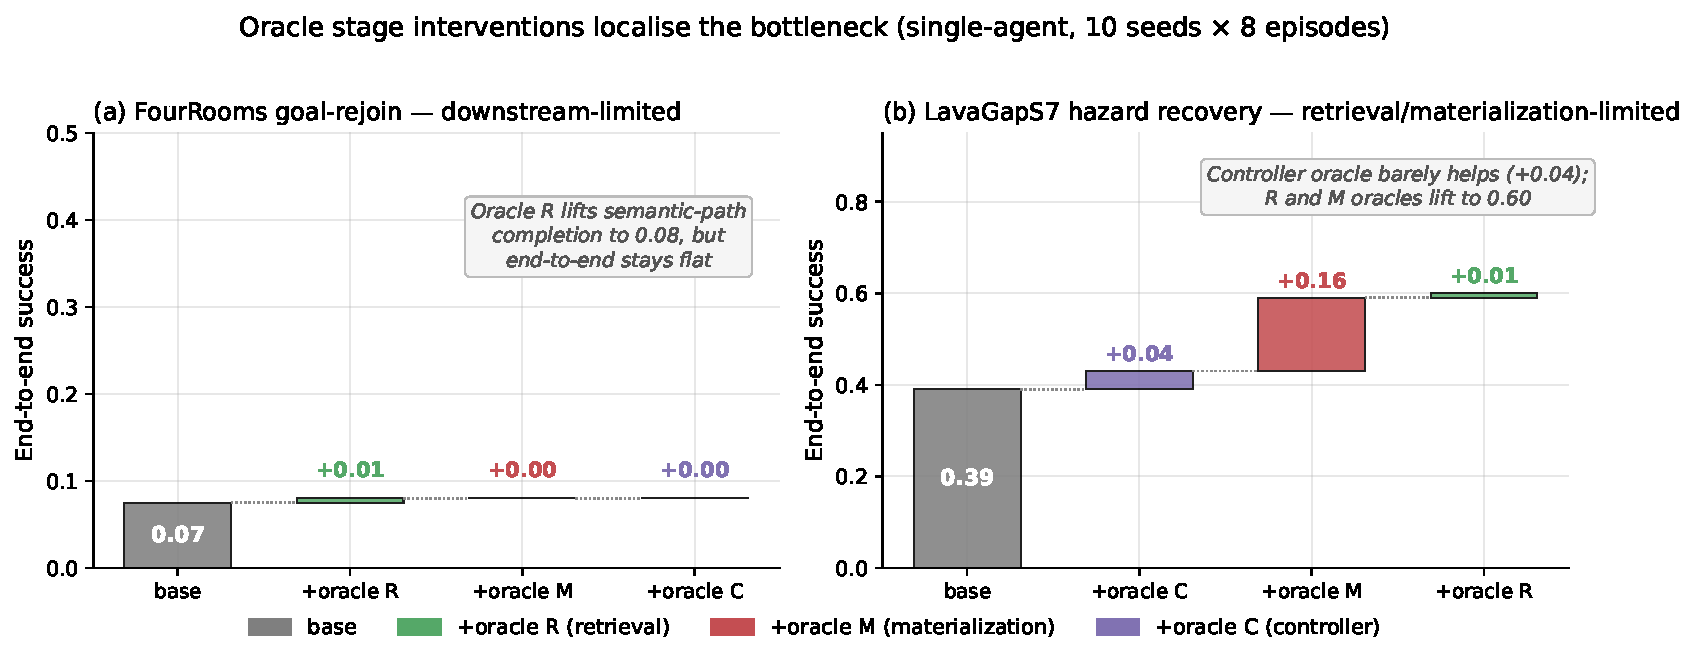
\includegraphics[width=0.98\columnwidth]{figures/fig_oracle_waterfall.pdf}
  \caption{Цикл диагноз$\to$вмешательство$\to$проверка на
  одноагентном бенчмарке: оракульные вмешательства на уровне этапов
  поднимают ровно тот этап, на который указывает декомпозиция.
  Восстановление после опасности ограничено извлечением (оракул-R:
  $0.39\!\to\!0.60$ сквозного успеха); возврат в целевую область
  ограничен нижележащими этапами (оракул-R спасает завершение
  семантического пути, сквозной успех не меняется).}
  \label{fig:oracle}
\end{figure}

Обученный baseline с клонированием поведения иллюстрирует тезис о
наблюдаемости: конкурентоспособный успех при схлопнутой этапной
структуре (нет явного интерфейса запросов/локов), то есть сквозная
оптимизация разменивает ровно те события, которые аудирует протокол.

\section{Мультиагентность: память как общий ресурс}
\label{sec:multi}

\begin{figure*}[t]
  \centering
  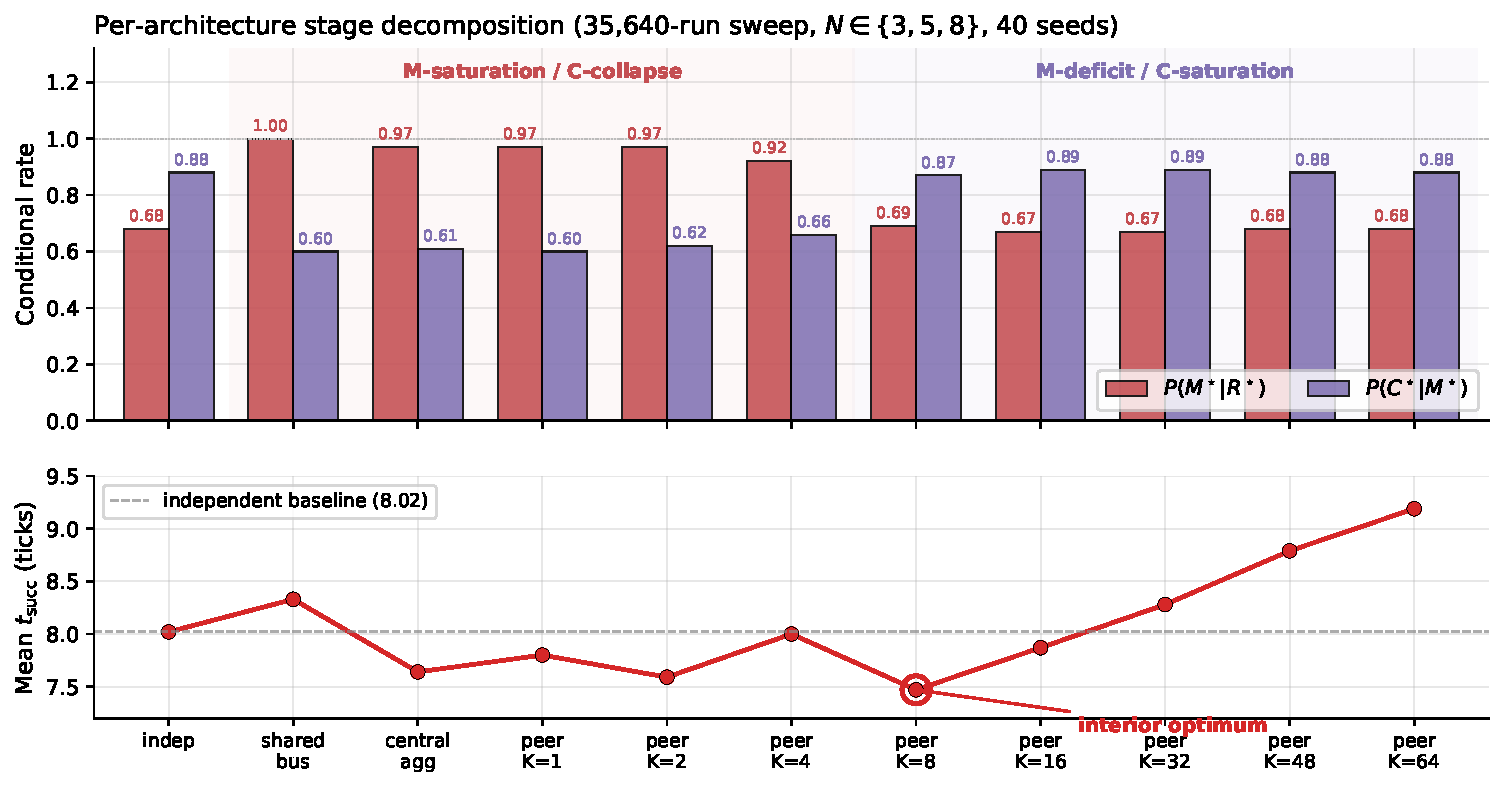
\includegraphics[width=0.92\textwidth]{figures/fig_conditional_rates.pdf}
  \caption{Условные частоты Q/R/M/C по архитектурам (сверху) и
  среднее время до успеха (снизу) на свипе из 35{,}640 прогонов.
  Общая шина, центральный агрегатор и быстрая пиринговая рассылка
  ($K{\le}4$) находятся в режиме насыщения M / коллапса C;
  независимые агенты и медленный пиринг ($K{\ge}16$) --- в обратном.
  Время до успеха имеет внутренний минимум при $K{=}8$ (7.47 против
  8.02 у независимых), устойчивый по положению, неглубокий по
  величине.}
  \label{fig:conditional-rates}
\end{figure*}

Четыре архитектуры обмена над одним символьным субстратом ---
независимые приватные памяти, общая шина событий, центральный
агрегатор со взвешиванием по доверию и пиринговая широковещательная
рассылка с каденцией $K{\in}\{1,\dots,64\}$ --- выполняют задачу
поиска дефицитной воды ($N{\in}\{3,5,8\}$ агентов, $T{\le}N$ целей,
три планировки, три плотности опасностей, 40 сидов; 35{,}640
прогонов). Рисунок~\ref{fig:conditional-rates} показывает этапный
профиль каждой архитектуры; извлечение насыщается, и вся
дифференциация живёт на звеньях M и C, как и предсказывает
Эмпирическое утверждение~1.

\textbf{Сдвиг узкого места.} По пиринговым прогонам коэффициент
Спирмена между $P(M^\star|R^\star)$ и $K$ равен $-0.53$
(кластерно-устойчивый 95\%-й ДИ $[-0.59,-0.47]$ по 81 конфигурационной
ячейке), а между $P(C^\star|M^\star)$ и $K$ равен $+0.43$
($[+0.37,+0.50]$). Более острая сигнатура --- внутрикаденционная:
коэффициент Пирсона между двумя звеньями внутри фиксированного $K$
достигает пика $-0.61$ при $K{=}4$ и затухает до шума к $K{=}64$ ---
узкое место мигрирует между этапами внутри одной и той же конфигурации
по мере изменения $K$. Масштабирование до $N{=}12$ \emph{заостряет}
сигнатуру (пик $-0.70$ с миграцией к $K{=}8$). На среднем времени до
успеха этот размен порождает внутренний оптимум при $K{=}8$; темп
консолидации --- реальная, настраиваемая ось проектирования.
Оракульные вмешательства замыкают цикл: при быстрой каденции
оракулы-R/M/C последовательно устраняют избыточное время, атрибутируя
его переходу M$\leftrightarrow$C.

\begin{figure}[t]
  \centering
  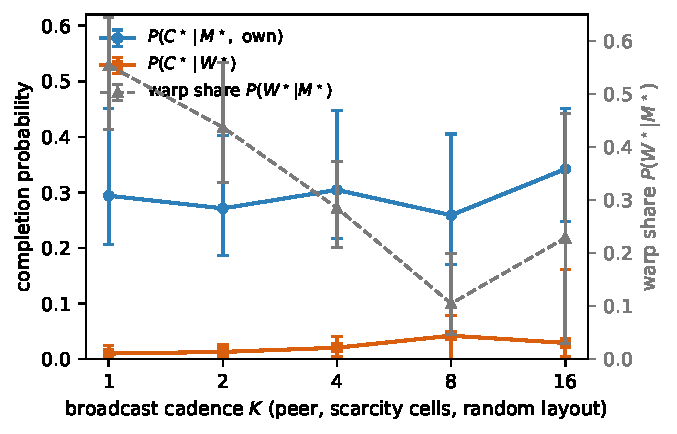
\includegraphics[width=0.98\columnwidth]{figures/fig_warp_strata.pdf}
  \caption{Стратификация $P(C^\star|M^\star)$ по провенансу в
  зависимости от каденции $K$ (пиринг, ячейки с дефицитом,
  бутстреп-ДИ с кластеризацией по эпизодам). Доля локов, опирающихся
  на чужие свидетельства (доля warp, серым), растёт с ускорением
  обмена, при этом завершение в этой страте (оранжевым) остаётся ниже
  $0.05$, а страта собственных свидетельств (синим) остаётся плоской:
  коллапс C при быстром обмене сосредоточен в страте чужих
  свидетельств.}
  \label{fig:strata}
\end{figure}

\textbf{Механизм --- провенанс.} Аннотируя каждое $M^\star$ долей
$\varphi$ чужих свидетельств в его опорной массе (вычисленной из
собственных весов слияния, замороженных в момент лока) и называя локи
с $\varphi{\ge}0.8$ \emph{warp}-локами: доля warp падает с $0.55$ при
$K{=}1$ до $0.11$ при $K{=}8$, тогда как локи на собственных
свидетельствах завершаются со стабильной частотой $0.26$--$0.34$, а
warp-локи --- ниже $0.05$ на всём диапазоне. Коллапс C при быстром
обмене концентрируется в страте чужих свидетельств --- каденция
управляет тем, какая часть коммитов коллектива опирается на
свидетельства напарников, и именно эта страта проигрывает гонку за
занятость. Та же кривая воспроизводится на непрерывном мосте VMAS
($0.72\!\to\!0.00$) и на текстовом LLM-субстрате
($0.42\!\to\!0.08$).

\textbf{Обученные и LLM-коллективы.} Baseline CommNet-PPO достигает
успеха символьного пиринга ($0.667$ против $0.65$) при структурно
вырожденных этапах (его вещественнозначный канал никогда не бывает
информативно пустым; R/M схлопываются) --- конкурентоспособный успех,
нулевая наблюдаемость этапов. Коллектив из трёх LLM-агентов
(llama3.1), разделяющих символьную память, воспроизводит
феноменологию на языке: при парном сравнении с baseline без
коммуникации на идентичных планировках сырой обмен \emph{снижает}
успех $2/3\!\to\!1/3$ (гонка за занятость), а децентрализованный
протокол резервирования с откатом возвращает часть его
($0.33\!\to\!0.42$) при латентности отката ${\approx}K$. На свипе по
бюджету шагов с двумя локальными моделями непрозрачный коллапс успеха
($1.00\!\to\!0.00$) разрешается в чистый сбой этапа C
($Q^\star{=}R^\star{=}M^\star{=}1$, $C^\star{=}0$) одинаково для
обеих моделей: диагноз структурный, а не модельно-специфичный.

\section{Контракт на сторонних агентных стеках}
\label{sec:external}

\begin{figure*}[t]
  \centering
  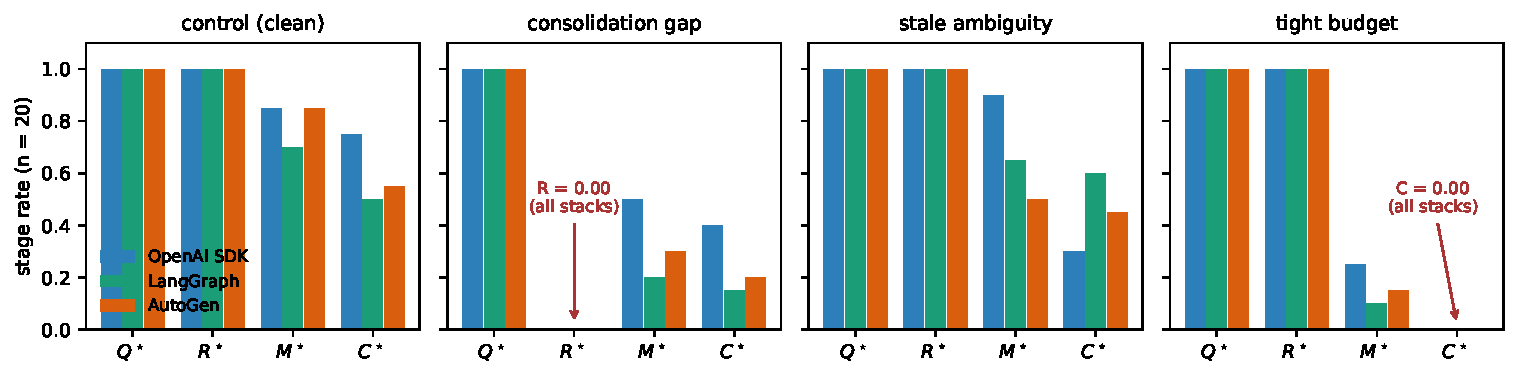
\includegraphics[width=0.92\textwidth]{figures/fig_external_stages.pdf}
  \caption{Этапные профили трёх сторонних стеков на четырёх
  сконструированных вариантах (llama3.1, $n{=}20$ на ячейку). Q и R
  насыщаются одинаково; структурные сбои дают точные нулевые столбцы
  на каждом стеке; межфреймворковый разброс живёт в M и C.}
  \label{fig:external-stages}
\end{figure*}

Работает ли протокол на системах, которые построили не мы? Мы
инструментируем три стека --- цикл function calling на OpenAI-SDK,
ReAct-агента LangGraph и AutoGen --- идентичным контрактом,
определённым единожды над \emph{трассами инструментов}: эпизодическая
бытовая память за инструментами
\method{recall}/\method{goto}/\method{take}; $Q^\star$ --- при
обращении с запросом, $R^\star$ --- при атрибуции (возвращённая
запись называет предмет в его истинном месте), $M^\star$ --- при локе
уровня эпизода, $C^\star$ --- при завершении в пределах бюджета
инструментов. Четыре варианта конструируют по одному сбою каждый; все
предсказания были зарегистрированы до прогонов, и две ревизии
семантики событий зафиксированы в регистрации.

\begin{table}[t]
\caption{Q/R/M/C на сторонних стеках (20 эпизодов на ячейку). $M_1$:
первый коммит нацелен на истинное место.}
\label{tab:external}
\centering
\small
\setlength{\tabcolsep}{3.4pt}
\begin{tabular}{llccccc}
\toprule
Стек & Вариант & $Q^\star$ & $R^\star$ & $M^\star$ & $C^\star$ & $M_1$ \\
\midrule
OpenAI & контроль      & 1.00 & 1.00 & .85 & .75 & .25 \\
SDK    & разрыв консол. & 1.00 & \textbf{.00} & .50 & .40 & .25 \\
       & уст.\ неодноз. & 1.00 & 1.00 & .90 & .30 & .25 \\
       & жёсткий бюджет & 1.00 & 1.00 & .25 & \textbf{.00} & .25 \\
\midrule
Lang-  & контроль      & 1.00 & 1.00 & .70 & .50 & .50 \\
Graph  & разрыв консол. & 1.00 & \textbf{.00} & .20 & .15 & .10 \\
       & уст.\ неодноз. & 1.00 & 1.00 & .65 & .60 & .50 \\
       & жёсткий бюджет & 1.00 & 1.00 & .10 & \textbf{.00} & .10 \\
\midrule
Auto-  & контроль      & 1.00 & 1.00 & .85 & .55 & .45 \\
Gen    & разрыв консол. & 1.00 & \textbf{.00} & .30 & .20 & .15 \\
       & уст.\ неодноз. & 1.00 & 1.00 & .50 & .45 & .35 \\
       & жёсткий бюджет & 1.00 & 1.00 & .15 & \textbf{.00} & .15 \\
\bottomrule
\end{tabular}
\end{table}

Три результата (таблица~\ref{tab:external},
рис.~\ref{fig:external-stages}). \textbf{(1)~Структурные локализации
точны и независимы от фреймворка}: нет консолидированного факта
$\Rightarrow R^\star{=}0.00$; бюджет ниже необходимого
$\Rightarrow C^\star{=}0.00$ при $Q^\star{=}R^\star{=}1$ --- $20/20$
эпизодов на каждом стеке, без адаптации под фреймворк.
\textbf{(2)~Чистый контроль разделяет стеки, а этапы говорят, чем
именно.} Успех на идентичных чистых эпизодах разбросан в диапазоне
$0.50$--$0.75$. Лидерборд сообщил бы <<разное качество>>; этапы
показывают общую патологию --- дисциплина первого коммита слаба
повсюду ($M_1{=}0.25$--$0.50$: первый \method{goto} часто игнорирует
только что извлечённые агентом собственные свидетельства) --- плюс
разную экономику циклов: M уровня эпизода восстанавливается до
$0.70$--$0.85$ повторным запросом, а стеки различаются тем, сколько
из этого доживает до завершения ($C/M$ от $0.88$ вниз до $0.65$).
\textbf{(3)~Устаревший дистрактор притягивает, и неравномерно.}
Устаревшая запись захватывает первый коммит в $0.20$--$0.40$
неоднозначных эпизодов, а её цена для завершения специфична для
фреймворка (OpenAI SDK: $0.75\!\to\!0.30$; остальные поглощают крюк).
Зарегистрированные поведенческие предсказания, предполагавшие чистый
контроль, провалились \emph{потому, что сами стеки проваливают чистую
задачу на память в 25--50\% случаев}, --- результат~(2), доложенный
как зарегистрированные неудачи с механизмами.

\section{Связанные работы}

Линии когнитивных и семантических карт мотивируют явную абстракцию
мест \citep{tolman1948cognitive,gupta2017cognitive,
savinov2018semi}; целеобусловленный RL обусловливается на цели или
эмбеддинги \citep{andrychowicz2017hindsight}; многоагентный RL
изучает обучаемые каналы \citep{sukhbaatar2016commnet,foerster2018ctde}
и госсип-протоколы \citep{boyd2006gossip}; системы LLM-агентов
добавляют явные слои памяти, оцениваемые сквозным образом
\citep{wang2023voyager,shinn2023reflexion,packer2023memgpt,
park2023generative,wu2023autogen}. Протокол ортогонален всем четырём
линиям: он не предлагает архитектуру; он делает любую из них
поэтапно диагностируемой по логам и даёт проверяемое на этих логах
предсказание о каденции на уровне наклонов.

\section{Ограничения}

Основные субстраты --- сеточные миры; VMAS --- ориентировочная
проверка в непрерывных состояниях; LLM-исследования используют
небольшие локальные модели при скромных $n$; идентичность мест между
агентами предполагает общую систему координат (конструктивно
устранено в сопутствующей рукописи); Эмпирическое утверждение~1
остаётся на уровне наклонов --- вывод при порождающей модели сделал
бы из него теорему. Полные таблицы, доказательства аргументов
оцениваемости, стресс-тесты предположений, методология размеров
эффекта, масштабирование и все файлы зарегистрированных предсказаний
--- в дополнении.

\section{Заключение}

Q/R/M/C превращает <<память агента отказала>> из скалярного вердикта
в локализованный, сопоставимый и порой исправимый диагноз: предел
консолидации у одиночного агента, темп обмена с ценой занятости в
коллективе, разрыв в дисциплине коммита у готовых агентных стеков.
Протокол стоит контракта логирования, а не новой архитектуры --- и те
же четыре числа читаются на символьных, обученных и LLM-системах.

\bibliography{aaai27refs}

% Чек-лист воспроизводимости не включается в русский дубль.
% \def\isChecklistMainFile{}
% \input{ReproducibilityChecklist_qrmc_aaai27.tex}

\end{document}
